Hasta ahora hemos estudiado la transmisión de símbolos digitales utilizando pulsos de banda base, que son apropiados para canales que responden adecuadamente a dichas frecuencias. Por ejemplo, el par trenzado de cobre o el cable coaxial, usado por ejemplo en Ethernet o en USB. Sin embargo, muchas veces, hace falta modular los datos digitales en otras partes del espectro, ya sea porque el medio así lo requiere (por ejemplo: enlaces satelitales o de terrestres de microondas, que utilizan señales de $\unit{\giga\hertz}$, WiFi, etc.), o por la necesidad de utilizar muchos canales dentro del mismo medio (ej: televisión digital sobre cable coaxial).

En principio, una solución posible sería modular tomar la onda PAM $x(t)=\sum_k a_k p(t-kT_s)$ generada por un modulador digital de banda base, y modularla de forma analógica en frecuencia, utilizando cualquier técnica de las vistas anteriormente como AM, FM, etc. Esto es conceptualmente correcto, pero no necesariamente es lo más eficiente. El hecho de que las señales sean digitales hace que pueda convenir combinar la modulación digital y la modulación pasabanda en un mismo proceso: desde el punto de vista de la modulación esto puede pensarse como que utilizamos \emph{pulsos de radiofrecuencia} $p_{\textrm{RF}}(t)$ para generar $x_{\textrm{RF}}(t)$, una señal digital modulada con espectro en la región de frecuencias deseada. Las dos interpretaciones son complementarias, como veremos.

Una segunda observación es que, desde el punto de vista de la detección, no es necesario volver a demodular completamente la señal (como sí lo requiere la transmisión analógica, por ejemplo FM comercial) sino simplemente \emph{detectar} el símbolo enviado mediante un muestreo y detección adecuados.

Consideremos una sinusoide base portadora $\cos(2\pi f_c t)$ a modular utilizando símbolos. Podemos cambiar varias características de la onda base para lograr enviar los datos digitales, por ejemplo:
\begin{description}
    \item[Amplitud:] 
    \begin{equation*}
        x_c(t) = a_k \cos(2\pi f_c t), \quad t\in[kT_s,(k+1)T_s],
    \end{equation*}
    con la amplitud codificando los símbolos
    \item[Fase:] 
    \begin{equation*}
        x_c(t) = \cos(2\pi f_c t + \theta_k), \quad t\in[kT_s,(k+1)T_s],
    \end{equation*}
    con $\theta_k$ codificando los símbolos.
    \item[Frecuencia: ] 
    \begin{equation*}
        x_c(t) = a_k \cos\left(2\pi (f_c+a_kf_{\Delta}) t\right), \quad t\in[kT_s,(k+1)T_s],
    \end{equation*}
     con la variación en frecuencia $a_kf_{\Delta}$ codificando los símbolos.
\end{description}
En la Figura \ref{fig:ejemplos pasabanda} se muestran tres modulaciones de este tipo, junto con la modulación banda base del mismo mensaje utilizando pulsos NRZ. Cuando la señal digital afecta uno solo de estos parámetros, se habla de \emph{keying} (por analogía a las llaves discretas de la telegrafía), dando lugar a los llamados \emph{Amplitude Shift Keying (ASK)}, \emph{Phase Shift Keying (PSK)} y \emph{Frequency Shift Keying (FSK)}. Obviamente podemos combinar varias de estas estrategias simultáneamente como veremos.

\begin{figure}
    \begin{center}
    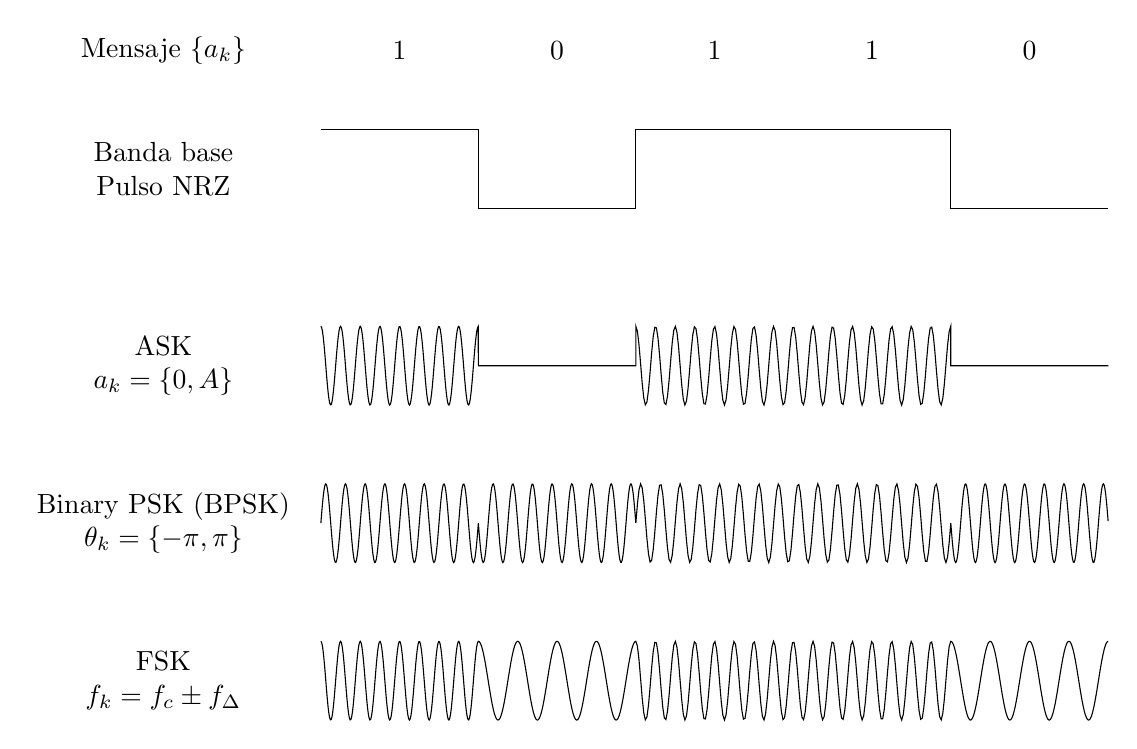
\begin{tikzpicture}
        \node[align=center] at (-2,1) {Mensaje $\{a_k\}$};
        \path (1,1) node {$1$} -- (3,1) node {$0$} -- (5,1) node {$1$} -- (7,1) node {$1$} -- (9,1) node {$0$};
        \begin{scope}[shift={(0,-1)}]
            \node [align=center] at (-2,.5) {Banda base\\Pulso NRZ};
            \draw (0,1) -- (2,1) -- (2,0) -- (4,0) -- (4,1) -- (8,1) -- (8,0) -- (10,0);
        \end{scope}
        \begin{scope}[shift={(0,-3)}]
            \node [align=center] at (-2,0) {ASK\\$a_k=\{0,A\}$};
            \draw [samples=200,domain=0:2] plot (\x,{.5*cos(8*pi*\x r)}) -- (2,0) -- (4,0) -- plot [samples=200,domain=4:8] (\x,{.5*cos(8*pi*\x r)}) -- (8,0) -- (10,0);
        \end{scope}
        \begin{scope}[shift={(0,-5)}]
            \node [align=center] at (-2,0) {Binary PSK (BPSK)\\$\theta_k=\{-\pi,\pi\}$};
            \draw [samples=200,domain=0:2] plot (\x,{.5*sin(8*pi*\x r)}) -- plot [domain=2:4] (\x,{-.5*sin(8*pi*\x r)}) -- plot [samples=200,domain=4:8] (\x,{.5*sin(8*pi*\x r)}) -- plot [domain=8:10] (\x,{-.5*sin(8*pi*\x r)});
        \end{scope}
       \begin{scope}[shift={(0,-7)}]
            \node [align=center] at (-2,0) {FSK\\$f_k=f_c\pm f_\Delta$};
            \draw [samples=200,domain=0:2] plot (\x,{.5*cos(8*pi*\x r)}) -- plot [domain=2:4] (\x,{.5*cos(4*pi*\x r)}) -- plot [samples=200,domain=4:8] (\x,{.5*cos(8*pi*\x r)}) -- plot [domain=8:10] (\x,{.5*cos(4*pi*\x r)});
        \end{scope}
    \end{tikzpicture}
    \end{center}
    \caption{Ejemplos de modulación digital pasabanda y comparación con banda base.}\label{fig:ejemplos pasabanda}
\end{figure}

Como veremos a continuación, los casos de ASK (también llamado ON-OFF keying, OOK, en el caso binario) y BPSK (Binary Phase Shift Keying) corresponden a una modulación lineal (al igual que la modulación AM o DSB). En cambio en FSK la dependencia es no lineal, como en el caso de FM.

\section{Modulación pasabanda binaria}

Sea entonces $\{a_k\}$ un proceso estocástico de tiempo discreto de símbolos binarios independientes e idénticamente distribuidos, y consideremos la onda digital de radiofrecuencia:
\begin{equation}\label{eq:onda PAM RF}
x_c(t) = \sum_k a_k p(t-kT_s) \cos(2\pi f_c t + \theta),    
\end{equation}
donde $p(t)$ es un pulso de banda base (ej: NRZ) y $\theta\sim\textrm{Uniforme}[0,2\pi]$ una fase aleatoria\footnote{En lo que sigue omitiremos esta fase aleatoria.}, que indica que el oscilador no necesariamente está sincronizado con los símbolos. Entonces $x_c(t)$ es una onda PAM de radiofrecuencia.

Observemos que la onda de la ecuación \eqref{eq:onda PAM RF} corresponde a realizar una modulación DSB de la onda PAM de banda base $x(t)=\sum_k a_k p(t-kT_s)$. Por lo visto en la Sección \ref{sec:modulacion wss}, podemos calcular el espectro de la onda $x_c$ como:
\begin{equation}\label{eq:dep PAM RF}
    S_{x_c}(f) = \frac{S_x(f-f_c) + S_x(f+f_c)}{4},
\end{equation}
donde recordamos la expresión para la densidad espectral de potencia en banda base \eqref{eq:dep onda pam iid}:
\begin{equation*}
S_x(f) = \sigma_a^2 f_s |\hat{P}(f)|^2 + \mu^2 f_s^2 \sum_{n=-\infty}^{+\infty} |\hat{P}(n f_s)|^2\delta(f-nf_s).    
\end{equation*}
Aquí $\mu$ y $\sigma_a^2$ son la media y varianza, respectivamente, de los símbolos $\{a_k\}$, y $\hat{P}(f)$ la transformada de Fourier del pulso de banda base.

Apliquemos el resultado anterior para analizar el espectro de diferentes modulaciones simples binarias.

\begin{ejemplo}[ON-OFF Keying (OOK), modulación ASK binaria]
    Este es el caso más simple, corresponde a utilizar un pulso de RF de amplitud $A$ para indicar un símbolo y ausencia de pulso para indicar el otro (ver Figura \ref{fig:ejemplos pasabanda}). Podemos identificar este esquema con la onda \eqref{eq:onda PAM RF} utilizando:
    \begin{equation*}
        a_k \in \{0,A\}, \quad p(t)=p_{[0,T_s]}(t)
    \end{equation*}
    es decir, en banda base, la modulación OOK se ve como una modulación binaria unipolar $\{0,A\}$ con pulsos NRZ.

    De lo visto en banda base, sabemos que $\mu = A/2$ y $\sigma_a^2=A^2/4$. A su vez $|\hat{P}(f)|^2= T_s \sinc(\pi f_s t)$ por lo que el espectro de $x(t)$ es:
    \begin{equation*}
        S_x(f) = \frac{A^2 T_s}{4} \sinc^2(\pi f_s t) + \frac{A^2}{4}\delta(f).
    \end{equation*}

    Utilizando entonces el resultado de modulación \eqref{eq:dep PAM RF} llegamos al siguiente espectro para la onda de RF, donde solo graficamos las frecuencias positivas:

    \begin{center}
    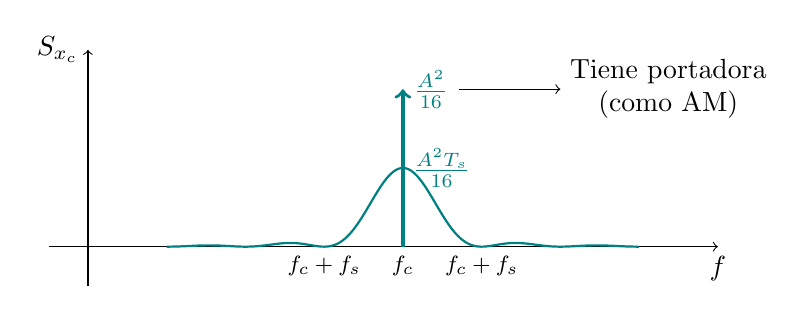
\begin{tikzpicture}
        \draw [->] (-0.5,0) -- (8,0) node [anchor=north] {$f$};
        \draw [->] (0,-0.5) -- (0,2.5) node[left] {$S_{x_c}$};
        \draw [teal,thick,samples=210,domain=1:7] plot (\x,{(sin(pi*(\x-4) r)/(pi*(\x-4)))^2});
        \node[teal,right] at (4,1) {$\frac{A^2 T_s}{16}$};
        \draw [very thick, teal, ->] (4,0) -- (4,2) node (a) [anchor=west] {$\frac{A^2}{16}$};
        \node [below] at (4,0) {\footnotesize $f_c$};
        \node [below] at (5,0) {\footnotesize $f_c+f_s$};
        \node [below] at (3,0) {\footnotesize $f_c+f_s$};
        \node [anchor=west, align=center] (b) at (6,2) {Tiene portadora\\(como AM)};
        \draw [->] (a) -- (b);
    \end{tikzpicture}
    \end{center}

    Notemos que esta modulación tiene ``portadora'' (como AM). A su vez, buena parte del espectro queda contenido a la banda $f_c\pm f_s$ por lo que si $f_c\gg f_s$, la señal ocupa una pequeña banda alrededor de la frecuencia de portadora. Esta señal es muy fácil de generar (y también de detectar como veremos), requiriendo únicamente encender y apagar un oscilador de RF. Es por ello que es ampliamente utilizada en aplicaciones sencillas, como por ejemplo, control remoto de dispositivos.
\end{ejemplo}


\begin{ejemplo}[Binary Phase Shift Keying (BPSK)]
    En este caso, el símbolo va codificado en la fase, es decir se transmite o bien $A\cos(2\pi f_c t)$ o bien $A\cos(2\pi f_c + \pi)$, de manera de separarlos lo más posible. Como $\cos(x+\pi) = -\cos(x)$, podemos identificar la onda PAM \eqref{eq:onda PAM RF} con la siguiente onda en banda base:
    \begin{equation*}
        a_k \in \{-A,A\}, \quad p(t) = p_{[0,T_s]}(t),
    \end{equation*}
    es decir, BPSK corresponde a utilizar en banda base una onda binaria polar NRZ. Nuevamente, por lo visto en banda base:
    \begin{equation*}
        S_x(f) = A^2 T_s \sinc^2(\pi f_s t),
    \end{equation*}
    de donde obtenemos el siguiente espectro de radiofrecuencia:
    \begin{center}
    \begin{tikzpicture}
        \draw [->] (-0.5,0) -- (8,0) node [anchor=north] {$f$};
        \draw [->] (0,-0.5) -- (0,2.5) node[left] {$S_{x_c}$};
        \draw [teal,thick,samples=210,domain=1:7] plot (\x,{2*(sin(pi*(\x-4) r)/(pi*(\x-4)))^2});
        \node[teal,right] at (4,2) {$\frac{A^2 T_s}{4}$};
        \node [below] at (4,0) {\footnotesize $f_c$};
        \node [below] at (5,0) {\footnotesize $f_c+f_s$};
        \node [below] at (3,0) {\footnotesize $f_c+f_s$};
    \end{tikzpicture}
    \end{center}

    Este es el ejemplo más sencillo de modulación digital eficiente en RF. En particular no tiene portadora. Nuevamente, la mayor parte de la potencia se encuentra concentrada en $f_c \pm f_s$, aunque al igual que en ASK, el ancho de banda es en principio infinito. Esto puede traer problemas de interferencia a bandas adyacentes así como ISI en la detección, como veremos.
\end{ejemplo}

\begin{ejemplo}[Binary Phase Shift Keying (BPSK) con pulsos de Nyquist]\label{ej:bpsk nyquist}
    Si queremos \emph{limitar} el ancho de banda de la señal BPSK, notemos que no es estrictamente necesario en la modulación utilizar un pulso cuadrado NRZ. Si cambiamos $x(t)$ por:
    \begin{equation*}
        x(t) = \sum_k a_k p(t-kT_s)
    \end{equation*}
    con $p(t)$ un pulso de Nyquist de exceso de ancho de banda $\alpha$, entonces la señal de banda base tiene densidad espectral acotada a la banda $\pm \frac{f_s}{2}(1+\alpha)$. Por lo tanto, la señal $x_c$ estará completamente contenida en la banda $f_c\pm \frac{f_s}{2}(1+\alpha)$ permitiendo ``encajar'' la onda en un canal acotado.

    \begin{center}
    \begin{tikzpicture}
        \draw [->] (-0.2,0) -- (8,0) node [anchor=north] {$f$};
        \draw [->] (0,-0.2) -- (0,2.5) node [anchor=west] {$S_{x_c}(f)$};
        \begin{scope}[shift={(4,0)}]
                \draw [teal, thick, samples=200,domain=-1.25:-0.75] plot (\x,{(1+cos(2*pi*(\x-0.25) r))}) -- (0.75,2);
                \draw [teal, thick, samples=200,domain=0.75:1.25] plot (\x,{(1+cos(2*pi*(\x+0.25) r))});
                \node[anchor=south west, teal] at (0,2) {$A^2\frac{T_s}{4}$};
                \node[below] at (0,0) {\footnotesize $f_c$};
                \node[below] at (1.25,0) {\footnotesize $f_c+\frac{f_s}{2}(1+\alpha)$};
                \draw[dotted] (1.25,0) -- (1.25,2);
                \draw[dotted] (-1.25,0) -- (-1.25,2);
                \draw[dashed] (0,0) -- (0,2);
        \end{scope}
    \end{tikzpicture}
    \end{center}

    La Figura \ref{fig:bpsk nyquist} muestra la forma de onda resultante, que es más complicada de generar que simplemente controlar un oscilador. Sin embargo, permite controlar el ``spillover'' de frecuencia (interferencia a bandas adyacentes) por lo cual este tipo de pulso es utilizado en la TV digital así como en la transmisión de datos RDS (Radio Data System) que envía datos digitales sobre las emisiones de radio FM comercial.
\end{ejemplo}
 
\begin{figure}    
    \begin{center}
        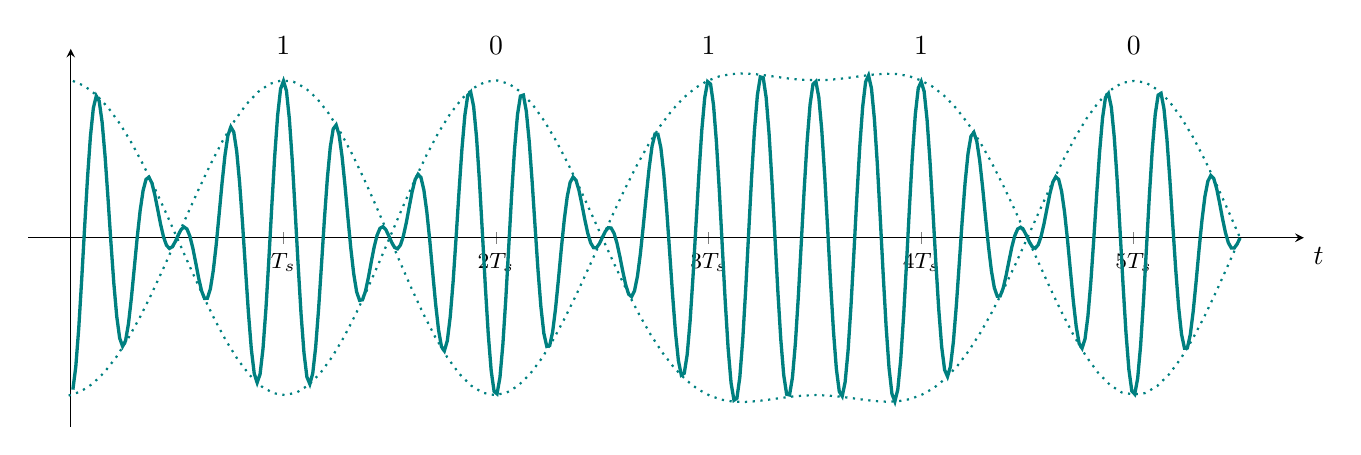
\begin{tikzpicture}
            \begin{axis}[ x=2.7cm, y=2cm, axis lines=middle,  
                every x tick label/.append style={font=\footnotesize},
                xlabel=$t$,
                x label style={anchor=north west},
                ylabel=\empty,
                ytick=\empty,
                xmin=-.2,xmax=5.8,ymin=-1.2,ymax=1.2,
                xtick = {1,2,3,4,5},
                xticklabels = {$T_s$,$2T_s$,$3T_s$,$4T_s$, $5T_s$},
                clip=false,
                ]
                \pgfmathdeclarefunction{rcpulse}{1}{\pgfmathparse{cos(deg(pi*#1))/(1-(2*#1)^2)*sin(deg(pi*#1))/(pi*#1)}};
                \addplot[teal, thick, dotted, domain=-0.01:5.5, samples=100] {-rcpulse(\x) + rcpulse(\x-1) - rcpulse(\x-2) + rcpulse(\x-3) + rcpulse(\x-4) - rcpulse(\x-5) + rcpulse(\x-6)};
                \addplot[teal, thick, dotted, domain=0.01:5.5, samples=100] {-(-rcpulse(\x)+rcpulse(\x-1) - rcpulse(\x-2) + rcpulse(\x-3) + rcpulse(\x-4) - rcpulse(\x-5) + rcpulse(\x-6))};
                \addplot[teal, very thick, domain=0.01:5.5, samples=400] {(-rcpulse(\x) + rcpulse(\x-1) - rcpulse(\x-2) + rcpulse(\x-3) + rcpulse(\x-4) - rcpulse(\x-5) + rcpulse(\x-6) )*cos(deg(8*pi*\x))};
                \node[above] at (axis cs:1,1.1) {$1$};
                \node[above] at (axis cs:2,1.1) {$0$};
                \node[above] at (axis cs:3,1.1) {$1$};
                \node[above] at (axis cs:4,1.1) {$1$};
                \node[above] at (axis cs:5,1.1) {$0$};
                \end{axis}    
        \end{tikzpicture}
    \end{center}
    \caption{Onda BPSK con pulsos de Nyquist de exceso de ancho de banda $\alpha=1$.}\label{fig:bpsk nyquist}
\end{figure}

Los anteriores ejemplos corresponden a modulaciones lineales, donde simplemente el pulso digital modula a la portadora, como en DSB o modulación AM clásica. Un ejemplo de modulación \emph{no lineal} se presenta a continuación, aunque un análisis completo excede a los objetivos de este curso.

\begin{ejemplo}[Modulación Binaria en frecuencia, BFSK]
    En este caso, la información de los símbolos va en la frecuencia de la portadora, transmitiéndose:
    \begin{equation*}
        x_c(t) = \sum_k A p(t-kT_s) \cos(2\pi (f_c + f_k) t),
    \end{equation*}
donde $p(t)$ es el pulso NRZ (indicando que solo se activa $f_k$ durante un tiempo de símbolo $T_s$) y el desvío de frecuencia es $f_k=\pm f_\Delta$.

Una forma de interpretar lo anterior es pensar que tenemos dos ondas de OOK con distinta frecuencia, que se alternan en el tiempo de acuerdo al símbolo a transmitir (en lugar de una única que se activa para el símbolo $1$, como en OOK). Es de esperar entonces que el espectro contenga impulsos en las frecuencias $f_c\pm f_\Delta$ debido a esto. Sin embargo, como las ondas que ASK superpuestas no son independientes, no es tan sencillo como sumar sus espectros.

De hecho, un análisis riguroso es complejo de hacer. El caso más común es la Modulación de Sunde, donde se elige $f_\Delta = f_s/2$. Esta elección tiene la virtud de que no produce discontinuidades bruscas en la fase, y puede verse que el espectro equivalente en banda base satisface:
\begin{equation*} 
    S_{x}(f) = \frac{A^2}{4}\left[\delta\left(f-\frac{f_s}{2}\right)+\delta\left(f+\frac{f_s}{2}\right)\right] + \frac{4 A^2 T_s \cos^2(\pi T_s f)}{\pi^2 (4 T_s^2 f^2 - 1)^2}.
\end{equation*}

\begin{center}
\begin{tikzpicture}[xscale=2.0]
    \draw [->] (-3,0) -- (3,0) node [anchor=north] {$f$};
    \draw [->] (0,-0.5) -- (0,2.5);
    \draw [teal, thick, samples=400,domain=-2.5:2.5] plot (\x,{20*(cos(pi*\x r)/(pi*(4*\x^2-1)))^2});
    \draw [->,teal, thick] (-0.5,0) node [anchor=north] {$-\frac{f_s}{2}$} -- (-0.5,2.1);
    \draw [->,teal, thick] (0.5,0) node [anchor=north] {$\frac{f_s}{2}$} -- (0.5,2.1);
    \draw (-1.5,0.1) -- (-1.5,-0.1) node [anchor=north] {$-3\frac{f_s}{2}$};
    \draw (1.5,0.1) -- (1.5,-0.1) node [anchor=north] {$3\frac{f_s}{2}$};
\end{tikzpicture}
\end{center}

Lo importante aquí es que la onda FSK ocupa un mayor ancho de banda que las modulaciones lineales ASK, BPSK ($3f_s$ respecto a $2f_s$ para los lóbulos centrales) al igual que ocurría en FM por comparación a AM.

La modulación FSK resultó muy popular en los comienzos de la transmisión digital, debido a que simplemente requería alternar entre dos osciladores, y a su vez como el espectro para el caso de Sunde cae como $f^4$, tiene poca interferencia a bandas adyacentes en comparación a ASK o BPSK con pulsos NRZ. Fue utilizada en las primeras versiones de Bluetooth, pero hoy ha caído en desuso, siendo más común la utilización de BPSK en el caso sencillo (con pulsos de Nyquist para controlar el spillover) y sus generalizaciones $M-$arias.

\end{ejemplo}

Para finalizar esta sección, comentemos ahora el tema de la \emph{eficiencia espectral} de las modulaciones pasabanda. En todos los casos, como se comentó, el ancho de banda requerido es \emph{como mínimo el doble} que la correspondiente situación de banda base. Esto es evidente en los casos lineales, ya que corresponde a trasladar el espectro de banda base a la frecuencia de portadora, y es aún mayor en el caso de la FSK de Sunde. Por lo tanto, la eficiencia espectral en $\unit{\bps/\hertz}$ será la mitad (o menos).

A modo de ejemplo, si se utiliza BPSK con pulsos de Nyquist ideales ($\alpha=0$ en el Ejemplo \ref{ej:bpsk nyquist}), ocupa un ancho de banda $f_s$ y obtiene una eficiencia espectral igual a $1$ bit por $\unit{\hertz}$, comparado con $2$ en el caso de banda base. La única forma de compensar esto es enviando más bits por símbolo, es decir pasar a modulaciones $M$-arias, que estudiamos a continuación.
